\documentclass[12pt]{scrartcl}%{article} % Beginn der LaTeX-Datei
%Titel etc

\title{
\begin{flushright}
 
\includegraphics[scale=0.5]{HAW_Marke_RGB_300dpi.jpg}
\end{flushright}

\vspace{3cm}

IT-Systeme\\
Konzept
 
\vspace{3cm}

\LARGE Interaktive Videoinstallation mit\\
granularem Synthesizer
}

%\author{}
\date{05.  November 2023}

% Kopf- und Fußzeilen

\usepackage[headsepline,%footsepline
]{scrlayer-scrpage}
\pagestyle{scrheadings}
\clearpairofpagestyles


\ihead{05.11.2023}
\chead{IT Systeme}
\ohead{Konzept}
\ifoot{}
\cfoot{}
\ofoot{\pagemark}

%% twocolumn

\usepackage{amsmath,amssymb}  % erleichtert Mathe 
\usepackage{enumerate}% schicke Nummerierung

\usepackage{graphicx} % für Grafik-Einbindung
%\usepackage{hyperref}

\usepackage[german]{babel}
\usepackage[T1]{fontenc}
\usepackage{lmodern}
\usepackage{textcomp}
 % Einstellungen, wenn man deutsch schreiben will, z.B. Trennregeln
\usepackage[utf8]{inputenc}  % für Unix-Systeme
  % ermöglicht die direkte Eingabe von Umlauten und ß
  % evt. obige Zeile ersetzen durch
  % \usepackage[ansinew]{inputenc}  % für Windows
  % \usepackage[applemac]{inputenc} % für den Mac


%%%%%%%%%%%%%%%%%%%%%%%%%%%%%%%%%%%%%%%%%%%%%%%%%%%%%%%%%%%%%%%%%%
%
%  ntheorem
%
\usepackage[thmmarks,amsmath,hyperref,noconfig]{ntheorem} 
  % erlaubt es, Sätze, Definitionen etc. einfach durchzunummerieren.
\newtheorem{satz}{Satz}[section] % Nummerierung nach Abschnitten
\newtheorem{hilfssatz}[satz]{Hilfssatz}
\newtheorem{kor}[satz]{Korollar}

\theorembodyfont{\upshape}
\newtheorem{beispiel}[satz]{Beispiel}
\newtheorem{bemerkung}[satz]{Bemerkung}
\newtheorem{definition}[satz]{Definition} %[section]

\theoremstyle{nonumberplain}
\theoremheaderfont{\itshape}
\theorembodyfont{\normalfont}
\theoremseparator{.}
\theoremsymbol{\ensuremath{_\blacksquare}}
\newtheorem{beweis}{Beweis}
\qedsymbol{\ensuremath{_\blacksquare}}
%\theoremclass{LaTeX}
%
% Ende ntheorem
%
%%%%%%%%%%%%%%%%%%%%%%%%%%%%%%%%%%%%%%%%%%%%%%%%%%%%%%%%%%%%%%%%%%


%\pagestyle{empty}
%
% Ändern der bedruckten Fläche der Seite
% \addtolength{\textwidth}{3cm}  % Befehl mit zwei Argumenten
% \addtolength{\textheight}{3cm}
% \hoffset-2cm % verschiebt das Textfenster nach links
% \voffset-5mm % verschiebt das Textfenster nach oben
%
%\parindent=0pt %% keine Einzug zu Beginn von Abs\"atzen
%\parskip=2mm   %% erzeugt einen zusätzliche Zeilenabstand zwischen
                %% Absätzen. Nötig bei \parindent=0pt


%%%%%%%%%%%%%%%%%%%%%%%%%%%%%%%%%%%%%%%%%%%%%%%%%%%%%%%%%%%%%%%%%%
% ermöglicht, farbigen Text zu drucken.
\usepackage{color}
% Und nun werden die Farben definiert - daran können Sie nach Belieben selber rumspielen.
\definecolor{white}{rgb}{1,1,1}
\definecolor{darkred}{rgb}{0.3,0,0}
\definecolor{darkgreen}{rgb}{0,0.3,0}
\definecolor{darkblue}{rgb}{0,0,0.3}
\definecolor{pink}{rgb}{0.78,0.09,0.51}
\definecolor{purple}{rgb}{0.28,0.24,0.55}
\definecolor{orange}{rgb}{1,0.6,0.0}
\definecolor{grey}{rgb}{0.4,0.4,0.4}
\definecolor{aquamarine}{rgb}{0.4,0.8,0.65}

\usepackage[table]{xcolor}% http://ctan.org/pkg/xcolor
\usepackage{lipsum}
\usepackage{wrapfig}



\DeclareMathOperator{\GL}{GL} % einige Macro, siehe am Ende Abschn. 2
\newcommand{\N}{\mathbb{N}}
\newcommand{\Z}{\mathbb{Z}}
\newcommand{\Q}{\mathbb{Q}}
\newcommand{\R}{\mathbb{R}}
\newcommand{\C}{\mathbb{C}}
\newcommand{\cP}{{\mathcal P}} 


\begin{document}

\begin{titlepage}


\maketitle % erzeugt den Kopf


\vfill 

\begin{flushleft}
\begin{tabular}{rlll}
%\cline{1-3}
\textbf{Gruppe:} & Ariane Bachmann (2xxxxxx) & Benjamin Ghodsi-Moghaddam (2xxxxxx) & \hspace{5cm} \\
 & Bruno Bühler (2xxxxxx) & Dennis Jonca (2xxxxxxx) & \hspace{5cm} \\
 & Fabian Brunner (2xxxxxx) & Rafael Weber (2xxxxxx) & \hspace{5cm} \\
& Tanggo Simamora (2xxxxxx) & & \hspace{5cm} \\\\
%\cline{1-3}
\textbf{Studiengang:} & Meidentechnik B.Sc. WS 23/24 & \hspace{5cm} \\\\
%\cline{1-3}
\textbf{eingereicht bei:} & Malte Sanders & \hspace{5cm} \\ 
%\cline{1-3}
\end{tabular}
\end{flushleft}

\end{titlepage}

\tableofcontents

\newpage

\section{Einleitung}

Im Rahmen des Kurses für IT-Systeme entsteht ein interaktives Projekt. Studierende haben die Möglichkeit, sowohl Hard- als auch Software eigenständig auszuwählen, um ein individuelle Idee zu entwickeln und umzusetzen. Im Folgenden wird das Konzept des ''Visuellen Synthesizers'' präsentiert.

\section{Product Vision}

\begin{figure}[h]
   \begin{minipage}[b]{.4\linewidth}
      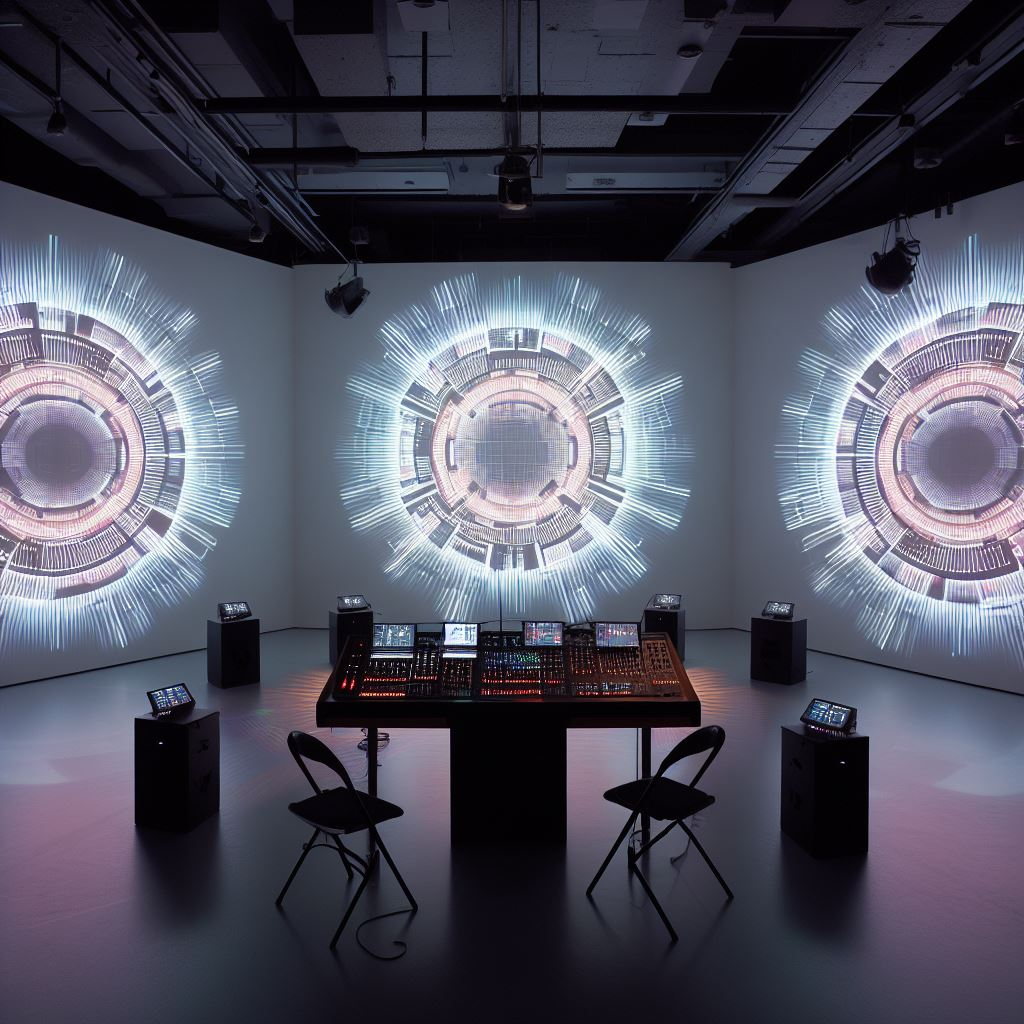
\includegraphics[width=\linewidth]{vision1}
      \caption{Projekt Vision:\\Rauminstallation}
   \end{minipage}
   \hspace{.1\linewidth}
   \begin{minipage}[b]{.4\linewidth}
      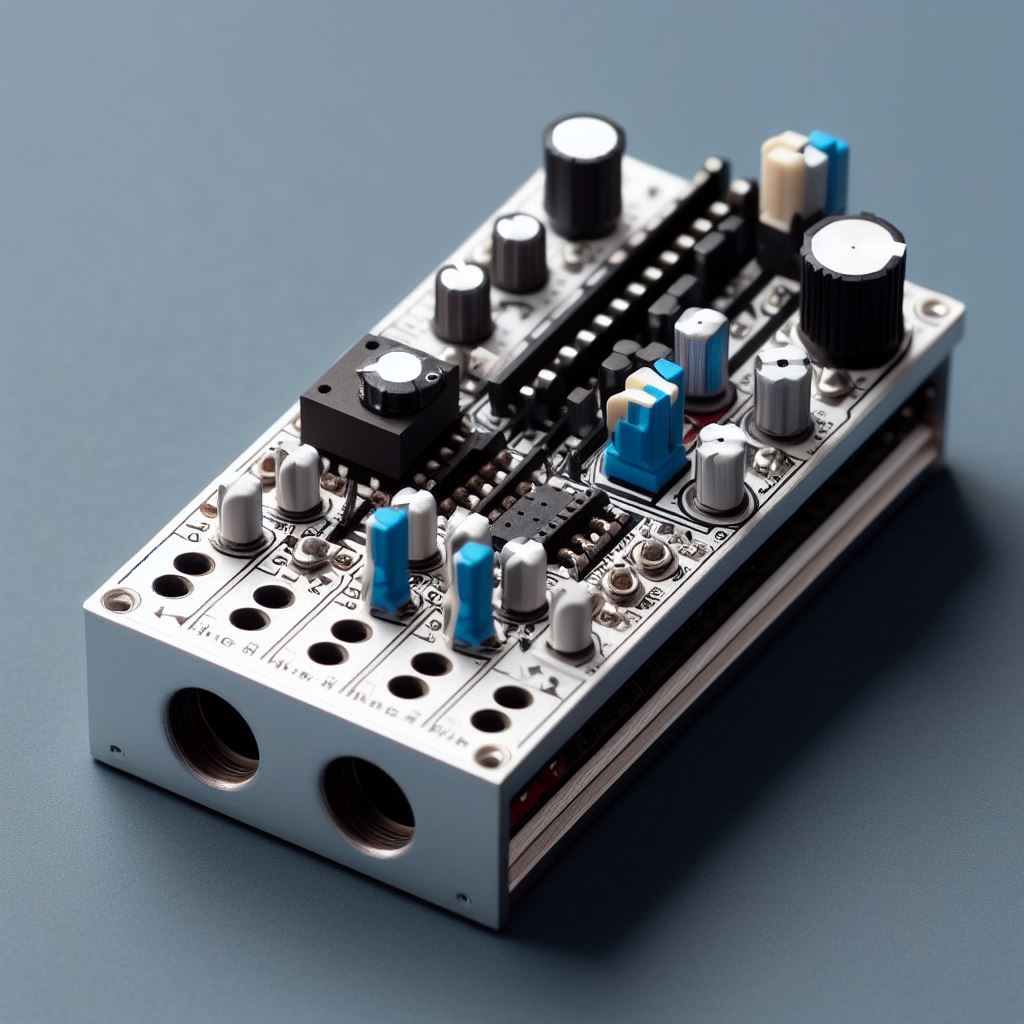
\includegraphics[width=\linewidth]{controller1}
      \caption{Projekt Vision:\\Synthesizer}
   \end{minipage}
\end{figure}
\noindent Die Idee ist es, eine Rauminstallation zu entwickeln, die kreativen Ausdruck und Interaktivität verbindet. Im Kern soll ein granularer Synthesizer stehen, der nicht nur außergewöhnliche Klänge erzeugt, sondern auch eine visuelle Dimension hinzufügt. Unabhängig vom Erfahrungsgrad der Nutzenden im Umgang mit Synthesizern und Videoanimation, tauchen diese in eine Welt voller künstlerischer Gestaltung. Durch die Kombination von Klangsynthese und visueller Darstellung ermöglichen wir es den Benutzenden, Klänge in Echtzeit zu formen und zu modulieren, während sie gleichzeitig die Wellenformen, Spektren und künstlerischen Visualisierungen dieser Klänge betrachten können.\\\\
Letztendlich soll der gesamte Raum zu einem Instrument verwandelt werden, in dem man isoliert von der Außenwelt eine ganz eigene Atmosphäre schafft und in ständiger Interaktion mit den visuellen und akustischen Eindrücken steht.
\newpage

\section{Systembeschreibung}

Die Systembeschreibung dient der Konkretisierung der Use-Cases sowie ihrer Umsetzung. Dabei werden die Anforderungen mithilfe der MoSCoW-Methode erläutert und die Komponenten der Umsetzung durch ein Systemabbild dargestellt.

\subsection{MoSCoW Priorisierung}

Die Hauptpriorität des Projekts liegt in der Erfüllung der Produktvision, die darauf abzielt, Audio und Video interaktiv zu gestalten. Während zahlreiche weitere Funktionen wünschenswert oder teilweise optional sind, ist es entscheidend, das Produkt so zugänglich wie möglich für Personen zu gestalten, die keine Erfahrung mit Synthesizern oder Videoanimation haben. Die Bedienung soll intuitiv und benutzerfreundlich gestaltet sein.
\begin{enumerate}[]
\item \textbf{Must}
  \begin{enumerate}[-]
  \item Die Synthese der Audiospur wird verarbeitet.
  \item Audiospur wird interaktiv durch die Nutzenden verändert.
  \item Die Interaktion wird durch digitale Visualisierungen dargestellt.
  \end{enumerate}
\item \textbf{Should}
  \begin{enumerate}[-]
  \item Die Aufnahme am Mikrofon wird zur Verarbeitung gespeichert.
  \item granulare Synthese mit den Parametern Grain Pitch, Grain Speed, Grain Scan und Reverb.
  \item Visualisierungen werden durch TouchDesigner entwickelt und wiedergegeben.
  \end{enumerate}
\item \textbf{Could}
  \begin{enumerate}[-]
  \item Die Aufnahme am Mikrofon wird in Echtzeit verarbeitet.
  \item Die entstandene Waveform der Audiospur kann für die Nutzenden angezeigt werden.
  \item Der Audio-Pitch kann an einem MIDI-Keyboard gesteuert werden.
  \item Es gibt mehrere Designs durch TouchDesigner.
  \item Die Nutzenden können aus mehreren Designs selbst wählen.
  \end{enumerate}
\item \textbf{Won't}
  \begin{enumerate}[-]
  \item zu viele Ablenkungen des Users (zweite GUI, etc.)
  \item zu komplexe Bedienung des Controllers für die Nutzenden.
  \end{enumerate}
\end{enumerate}

\subsection{Der Systemaufbau}

Die Nutzenden haben verschiedene Bedienungsmöglichkeiten zur Verfügung. Dazu gehören ein Mikrofon, dessen Aufnahmen als Grundlage für den Granular-Synthesizer dienen, Knöpfe zum Starten und Stoppen der Mikrofonaufnahme, Potentiometer und Slider, die die Steuerung der Synthesizer-Parameter ermöglichen, sowie ein MIDI-Keyboard zur Tonhöhenkontrolle des Synthesizers.\\\\
Zusätzlich könnte es eine Anzeige der aufgenommenen Audiospur in Form einer Waveform geben. Der Mikrocontroller und das Keyboard senden MIDI-Daten an einen Computer, auf dem die Audiosynthese der zuvor aufgenommenen Audiodatei stattfindet. Das resultierende Audiosignal wird zum einen über Lautsprecher im Raum wiedergegeben und zum anderen zusammen mit den MIDI-Daten an TouchDesigner weitergeleitet. Sowohl Audio als auch MIDI beeinflussen die Visualisierung, die über einen Beamer mittels HDMI in den Raum projiziert wird.
\begin{center}
 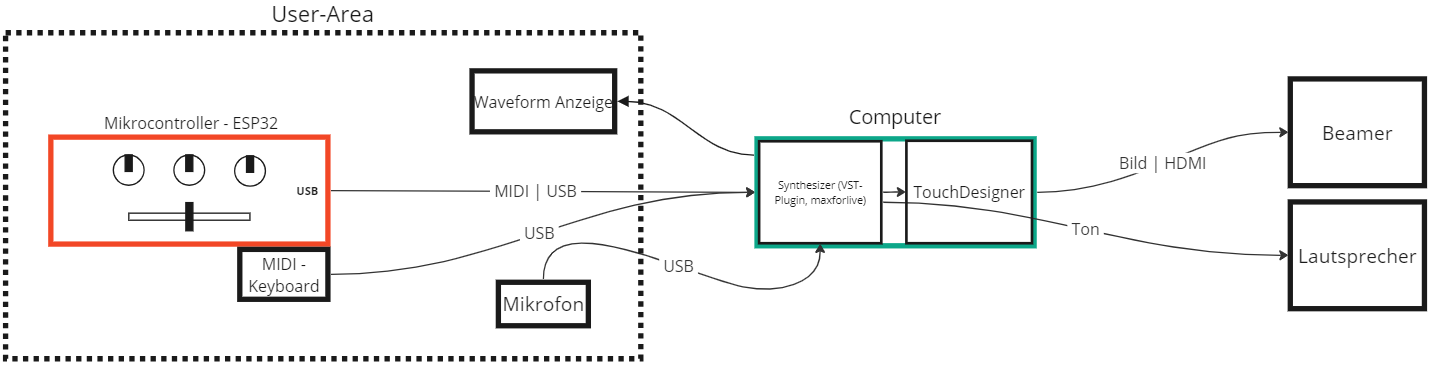
\includegraphics[scale=0.43]{system_schaltbild_v1.png}
 \captionof{figure}{Blockschaltbild des kompletten Systems}
\end{center}
\newpage
\subsection{Die Use Cases}
Eine Person tritt an die Installation heran und beginnt, Klänge durch die Verwendung des Mikrofons aufzunehmen. Mit den Poti's und Schiebereglern steuert die Person die Klang- und visuellen Effekte. Durch das MIDI-Keyboard werden die Töne gesteuert. Die aufgenommenen Audiospuren und manipulierten visuellen Effekte werden in Echtzeit wiedergegeben, sodass die Nutzenden eine unmittelbare kreative Interaktion erleben.
\begin{center}
 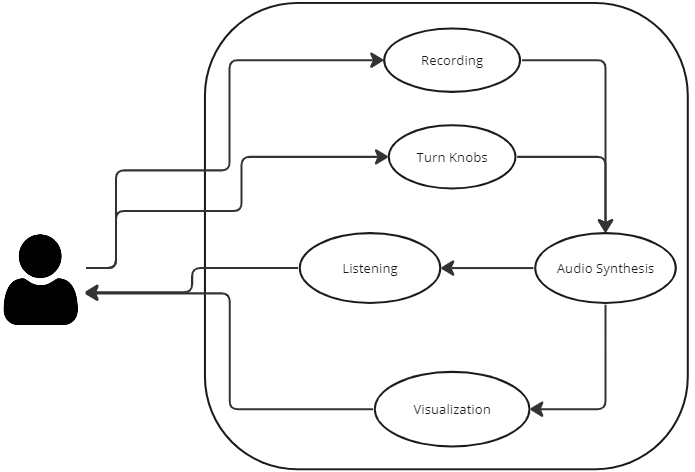
\includegraphics[scale=0.4]{usecases2.png}
 \captionof{figure}{Usecase Diagramm des Projekts}
\end{center}
\section{Roadmap}
Die Roadmap bietet einen zeitlichen Rahmen für das Projekt. Sie enthält alle Projektwochen und einen konzipierten Ablaufplan. Dieser kann sich gemäß den Prinzipien des agilen Projektmanagements während des Projekts verändern.
\begin{flushleft}
 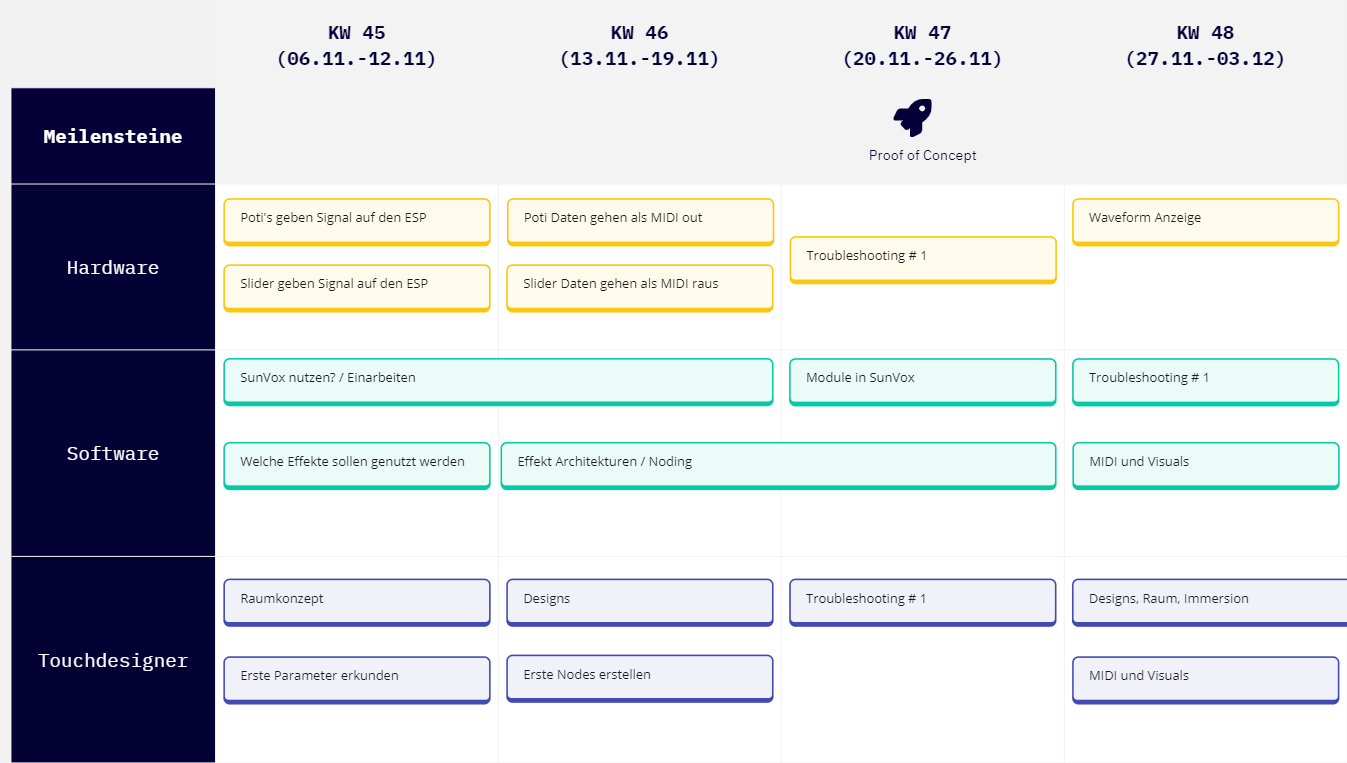
\includegraphics[scale=0.4]{road1.png}
 \captionof{figure}{Roadmap Teil 1}
\end{flushleft}
\begin{flushleft}
 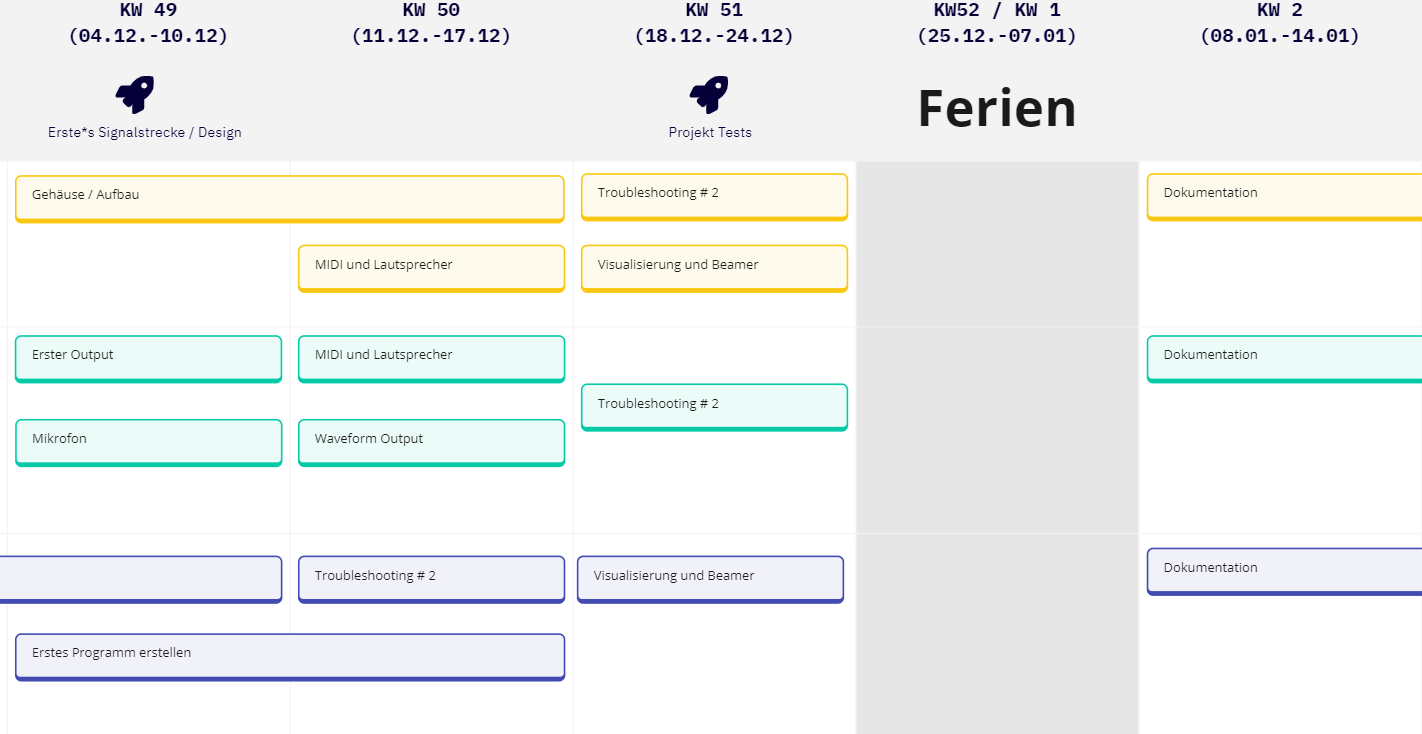
\includegraphics[scale=0.4]{road2.png}
 \captionof{figure}{Roadmap Teil 2}
\end{flushleft}
\begin{flushleft}
 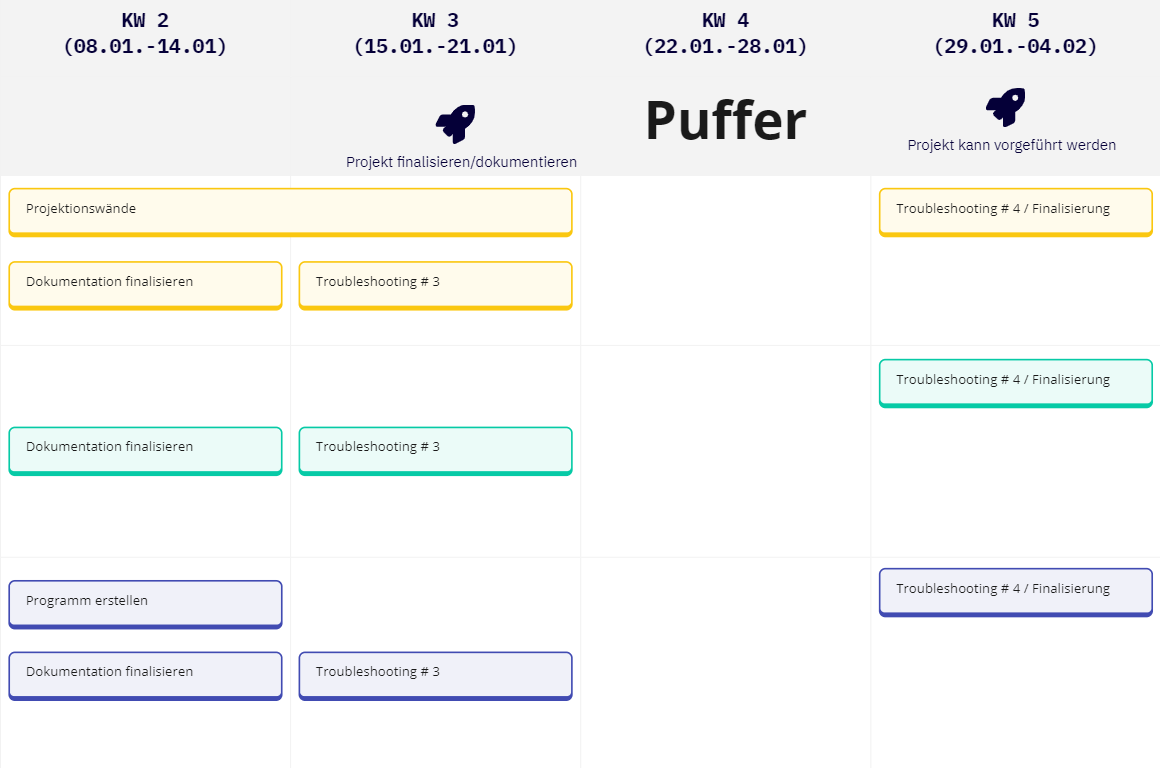
\includegraphics[scale=0.4]{road3.png}
 \captionof{figure}{Roadmap Teil 3}
\end{flushleft}

\end{document}